\documentclass{article}
\usepackage{wrapfig}
\usepackage{graphicx}
\usepackage{pdfpages}
\usepackage{nicematrix}
\usepackage{siunitx}
\usepackage{makecell}
\usepackage{multirow,bigdelim}
\usepackage{tikz}
\usetikzlibrary{decorations.pathreplacing,calc,tikzmark}

\begin{document}

\begin{center}
\begin{tabular}{c|c|c||c|c|c}
\multicolumn{6}{c}{TABLE VII}\\[3pt]
\hline
\hline
\rule{0pt}{1.5\normalbaselineskip}
$n$ & $4.917\!\times\!{n}$ & \makecell{\small{Observed}\\\small{Charge}} & $n$ & $4.917\!\times\!{n}$ & \makecell{\small{Observed}\\\small{Charge}}\\[8pt]
\hline
\rule{0pt}{1\normalbaselineskip}
1 & 4.917 & $\cdots$ & 10 & 49.17 & 49.41\\
2 & 9.834 & $\cdots$ & 11 & 54.09 & 53.91\\
3 & 14.75 & $\cdots$ & 12 & 59.00 & 59.12\\
4 & 19.66 & 19.66  & 13 & 63.92 & 63.68\\
5 & 24.59 & 24.60  & 14 & 68.84 & 68.65\\
6 & 29.50 & 29.62  & 15 & 73.75 & $\cdots$\\
7 & 34.42 & 34.47  & 16 & 78.67 & 78.34\\
8 & 39.34 & 39.38  & 17 & 83.59 & 83.22\\
9 & 44.25 & 44.42  & 18 & 88.51 & $\cdots$\\[3pt]
\hline
\end{tabular}
\end{center}

\bigskip

\begin{center}
\small
\begin{tabular}{|S|c||S|c|c|c|c|c|c|c|}
\hline
\rule{0pt}{1.5\normalbaselineskip}
 & $d$ = 0.5cm & & $d$ = 0.5cm & \makecell{Charge\\on ion} & & & \makecell{Frictional\\charge} & & \\[10pt]
\hline
\rule{0pt}{1.5\normalbaselineskip}
$t_g$ & \makecell{$v_1(=d/t_g)$\\(cm/sec)} & $t_F$ & \makecell{$v_2(=d/t_F)$\\(cm/sec)} & $(v_{2}'\!-\!v_2)$ & $n'$ & $\frac{v_{2}'-v_2}{n'}$ & $v_1+v_2$ & $n$ & $\frac{v_1+v_2}{n}$\\[10pt]
\hline
\rule{0pt}{1\normalbaselineskip}
18.2    & .00286 & 3.8 & .01316 & & & & .01602 & 3 & .00534\\
18.6    & \emph{avr}  & & & .00470 & 1 & .00470 & & & \\
19.2    & & 2.8 & .01786 & & & & & & \\
18.0    & & & & .01561 & 3 & .00520 & & & \\
17.2    & & 22.2 & .00225 & & & & & & \\
15.4    & & & & .00544 & 1 & .00544 & & & \\
16.7    & & 6.5 & .00769 & & & & & & \\
18.0    & & & & .00541 & 1 & .00541 & & & \\
15.4    & & 21.9 & .00228 & & & & & & \\
17.3    & & & & .01123 & 2 & .00562 & & & \\
18.4    & & 3.7 & .01351 & & & & & & \\[3pt]
\hline
\rule{0pt}{1\normalbaselineskip}
17.5 & & & & & & .00527 & & & .00534\\
{\makecell[l]{\emph{avr}}} & & & & & & \emph{avr} & & &\\[3pt]
\hline
\end{tabular}
\end{center}

\bigskip

\begin{table}[htp]
\centering
\begin{minipage}{\textwidth}
\centering
\begin{tabular}{c|r@{\hspace{10pt}}|l@{\hspace{10pt}}|l|c|c||c|c|c}
\multicolumn{9}{c}{TABLE VI\footnote{[The bracketed numbers are our corrections of errors in the original paper.]}}\\[3pt]
\hline\hline
\makecell{$t_g$\\[-2pt]\footnotesize{Sec.}} & \makecell{$t_{\scriptstyle{F}}$\\[-2pt]\footnotesize{Sec.}} & $\ \ \frac{1}{t_F}$ & $\frac{1}{t'_F}-\frac{1}{t_F}$ & $n'$ & $\frac{1}{n'}(\frac{1}{t'_F}-\frac{1}{t_F})$ & $\frac{1}{t_g}+\frac{1}{t_F}$ & n & $\frac{1}{n}(\frac{1}{t_g}+\frac{1}{t_F})$\\[5pt]
\hline
\rule{0pt}{1\normalbaselineskip}%space before first row numbers
11.848 & 80.708 & .01236\phantom{0}\tikzmark{3} & & & & .09655 & 18 & .005366\\
11.890 & 22.366\tikzmark{1} & & .03234 & 6 & .005390 & & & \\
11.908 & 22.390 & .04470\phantom{0}\tikzmark{4}\tikzmark{6} & & & & .12887 & 24 & .005371\\
11.904 & 22.368\tikzmark{2} & & .03751 & 7 & .005358 & & & \\
11.882 & 140.565 & .007192\tikzmark{5}\tikzmark{7}  & & & & .09138 & 17 & .005375\\
& & & .005348 & 1 & .005348 & & &\\
11.906 & 79.600 & .01254\phantom{0}\tikzmark{8} & & & & .09673 & 18 & .005374\\
11.838 & 34.748\tikzmark{9} & & .01616  & 3 & .005387 & & & \\
11.816 & 34.762 & .02870\phantom{0}\tikzmark{11}  & & & & .11289 & 21 & .005376\\
11.776 & 34.846\tikzmark{10} & & & & & & \\
11.840 & 29.286\tikzmark{12} & & & & & & \\
& & .03414\phantom{0}\tikzmark{20} & & & & .11833 & 22 & .005379 \\
11.904 & 29.236\tikzmark{13} & & .026872 & 5 & .005375 & & \\
11.870 & 137.308 & .007268\tikzmark{21} \\
& & & .021572 \\
11.952 & 34.638 & .02884\phantom{0}\tikzmark{22} \\
11.860 & & & .01623 \\
11.846 & 22.104\tikzmark{14} &\\
& & .04507\phantom{0}\tikzmark{23} \\
11.912 & 22.268\tikzmark{15} & & .04307 \\
11.910 & 500.1\phantom{00} & .002000\tikzmark{24}\\
11.918 & 19.704\tikzmark{16} & & .04879 \\
& & .05079\phantom{0}\tikzmark{25}\\
11.870 & 19.668\tikzmark{17} &\\
& & & .03874\\
11.888 & 77.630\tikzmark{18} &\\
& & .01285\phantom{0}\tikzmark{26}\\
11.894 & 77.806\tikzmark{19} & & .01079\\
11.878 & 42.302 & .02364\phantom{0}\tikzmark{27}\\
\hline
\rule{0pt}{0.8\normalbaselineskip}
$11.880\,\,$ \\
\hline
\end{tabular}
\small
\begin{tabular}{l@{\hskip 2em} l l@{\hskip 5em} l l}\\[-8pt]
& Duration of exp. & = 45 min. & Pressure & = 75.62 cm.\\
& Plate distance & = 16 mm. & Oil density & = .9199\\
& Fall distance & = 10.21 mm. & Air viscosity & = $1,824\times 10^{\,\text{-}7}$ [poise]\\
& Initial volts & = 5,088.8 & Radius ($a$) & = .000276 cm.\\
& Final volts & = 5,081.2 & $\frac{l}{a}$ [mean free path $\div\ a$] & = .034\\[2pt]
& Temperature & = 22.82\textdegree C. & Speed of fall & = .08584 cm./sec.\\[3pt]
\multicolumn{5}{c}{$e_i = 4.991\times 10^{\,\text{-}10}$ [statcoulomb]\footnote{[The value presently accepted is $4.802\times 10^{\,\text{-}10}$ statcoulombs.]}}\\
\end{tabular}
\begin{tikzpicture}[remember picture]
% Column 2 braces
\draw[overlay,decorate,
    decoration = {brace,raise=3pt,amplitude=4pt,aspect=0.45}]([shift={(0pt,2pt)}]pic cs:1) -- ([shift={(0pt,2pt)}]pic cs:2);
\draw[overlay,decorate,
    decoration = {brace,raise=3pt,amplitude=4pt,aspect=0.45}]([shift={(0pt,3pt)}]pic cs:9) -- ([shift={(0pt,2pt)}]pic cs:10);
\draw[overlay,decorate,
    decoration = {brace,raise=3pt,amplitude=4pt,aspect=0.45}]([shift={(0pt,3pt)}]pic cs:12) -- ([shift={(0pt,2pt)}]pic cs:13);
\draw[overlay,decorate,
    decoration = {brace,raise=3pt,amplitude=4pt,aspect=0.45}]([shift={(0pt,3pt)}]pic cs:14) -- ([shift={(0pt,2pt)}]pic cs:15);
\draw[overlay,decorate,
    decoration = {brace,raise=3pt,amplitude=4pt,aspect=0.45}]([shift={(0pt,3pt)}]pic cs:16) -- ([shift={(0pt,2pt)}]pic cs:17);
\draw[overlay,decorate,
    decoration = {brace,raise=3pt,amplitude=4pt,aspect=0.45}]([shift={(0pt,3pt)}]pic cs:18) -- ([shift={(0pt,2pt)}]pic cs:19);

% Column 3 braces
\draw[overlay,decorate,
    decoration = {brace,raise=2pt,amplitude=4pt,aspect=0.45}]([shift={(0pt,3pt)}]pic cs:3) -- ([shift={(0pt,3pt)}]pic cs:4);
\draw[overlay,decorate,
    decoration = {brace,raise=2pt,amplitude=4pt,aspect=0.45}]([shift={(0pt,3pt)}]pic cs:6) -- ([shift={(0pt,3pt)}]pic cs:5);
\draw[overlay,decorate,
    decoration = {brace,raise=2pt,amplitude=4pt,aspect=0.45}]([shift={(0pt,3pt)}]pic cs:7) -- ([shift={(0pt,2pt)}]pic cs:8);
\draw[overlay,decorate,
    decoration = {brace,raise=2pt,amplitude=4pt,aspect=0.45}]([shift={(0pt,2pt)}]pic cs:8) -- ([shift={(0pt,2pt)}]pic cs:11);
\draw[overlay,decorate,
    decoration = {brace,raise=2pt,amplitude=4pt,aspect=0.45}]([shift={(0pt,2pt)}]pic cs:20) -- ([shift={(0pt,2pt)}]pic cs:21);
    \draw[overlay,decorate,
    decoration = {brace,raise=2pt,amplitude=4pt,aspect=0.45}]([shift={(0pt,2pt)}]pic cs:21) -- ([shift={(0pt,2pt)}]pic cs:22);
    \draw[overlay,decorate,
    decoration = {brace,raise=2pt,amplitude=4pt,aspect=0.3}]([shift={(0pt,2pt)}]pic cs:22) -- ([shift={(0pt,2pt)}]pic cs:23);
    \draw[overlay,decorate,
    decoration = {brace,raise=2pt,amplitude=4pt,aspect=0.45}]([shift={(0pt,2pt)}]pic cs:23) -- ([shift={(0pt,2pt)}]pic cs:24);
    \draw[overlay,decorate,
    decoration = {brace,raise=2pt,amplitude=4pt,aspect=0.45}]([shift={(0pt,2pt)}]pic cs:24) -- ([shift={(0pt,2pt)}]pic cs:25);
    \draw[overlay,decorate,
    decoration = {brace,raise=2pt,amplitude=4pt,aspect=0.45}]([shift={(0pt,2pt)}]pic cs:25) -- ([shift={(0pt,2pt)}]pic cs:26);
    \draw[overlay,decorate,
    decoration = {brace,raise=2pt,amplitude=4pt,aspect=0.45}]([shift={(0pt,2pt)}]pic cs:26) -- ([shift={(0pt,2pt)}]pic cs:27);
\end{tikzpicture}
\end{minipage}
\end{table}

\begin{tabular}{r r r r}
\hline
1 & 2\tikzmark{A} & 3 & 4\\
5 & 6\tikzmark{D} & \tikzmark{B}7 & 8\\
9 & 10\tikzmark{C} & 11 & 12\\
\hline
\end{tabular}
\tikz[remember picture]
\draw[overlay,decorate,
    decoration = {brace,raise=6pt,amplitude=3pt,aspect=0.45}]([shift={(0pt,2pt)}]pic cs:A) -- ([shift={(0pt,2pt)}]pic cs:C);
\bigskip

\begin{tabular}{r r r r}
\hline
1 & 2\tikzmark{a} & 3 & 4\\
5 & 6\tikzmark{d} & \tikzmark{b}7 & 8\\
9 & 10\tikzmark{c} & 11 & 12\\
\hline
\end{tabular}
\tikz[remember picture]\draw[overlay]([shift={(1pt,2pt)}]pic cs:a) -- ([shift={(-2pt,4pt)}]pic cs:b);
\tikz[remember picture]\draw[overlay]([shift={(1pt,2pt)}]pic cs:c) -- ([shift={(-2pt,4pt)}]pic cs:b);

\bigskip

%\url{https://tex.stackexchange.com/a/1570/86}

\hfill\tikzmark{right}
\begin{itemize}
\item First line
\item Second line \tikzmark{2nd}
\item Third line, which is quite long and seemingly tedious in the extreme
\item Fourth line, which isn't as long as the third \tikzmark{4th}
\item Fifth line
\end{itemize}


\begin{tikzpicture}[overlay, remember picture]
\node[anchor=base] (a) at (pic cs:2nd) {\vphantom{h}}; % push the mark to the top of the line (ie including ascenders)
\node[anchor=base] (b) at (pic cs:4th) {\vphantom{g}}; % push the mark to the bottom of the line (ie including descenders)
\draw [decoration={brace,amplitude=0.5em},decorate,ultra thick,gray]
 (a.north -| {pic cs:right}) -- (b.south -| {pic cs:right});
\end{tikzpicture}

\begin{equation}
P(\pmb{a}, \pmb{b}) = \int d\lambda\, \rho(\lambda) A(\pmb{a}, \lambda) B(\pmb{b}, \lambda).\footnote{[According to the hypothesis Bell is investigating, the "more complete specification" of the particles' state, the extra information that would tell the observer who knew it which way the particle would respond to a given measurement, is given by $\lambda$. Equation (2) considers all the possible $\lambda$'s and weights them according to how likely each is. Mathematically, that means integrating over all the possible values of $\lambda$ and weighting each by its likelihood, represented by the probability distribution $\rho(\lambda)$. It may be helpful to note that $P$ was likely chosen to stand for "product," since the term we are integrating $\rho$ against is the product of $A$ and $B$. Because we've defined $A$ and $B$ such that the results of measurements yield the values $+1$ and $-1$, the product for any given value of $\lambda$ will always be either $+1$ (meaning that the two particles would both be measured to be pointing either in the selected directions $\pmb{a}$ and $\pmb{b}$ or in directions opposed to them) or $-1$ (meaning that the directions of $\pmb{\sigma}_1$ and $\pmb{\sigma}_2$ would be measured to be opposed, whether because $\pmb{\sigma}_1$ would \emph{not} be measured to point in direction $\pmb{a}$ and $\pmb{\sigma}_2$ \emph{would} be measured to point in direction $\pmb{b}$ or because $\pmb{\sigma}_1$ \emph{would} be measured to point in direction $\pmb{a}$ and $\pmb{\sigma}_2$ would \emph{not} be measured to point in direction $\pmb{b}$. Since it is weighted sum of all the positive and negative terms, $P(\pmb{a},\pmb{b})$ is thus a measure of the \emph{correlation} between the spin-direction of the two particles relative to the angles $\pmb{a}$ and $\pmb{b}$.]}
\end{equation}

\newpage

\section*{Note\\
  {\large Single-slit Diffraction and the Limit of Optical Resolution}}

\begin{wrapfigure}{r}{0.45\textwidth}
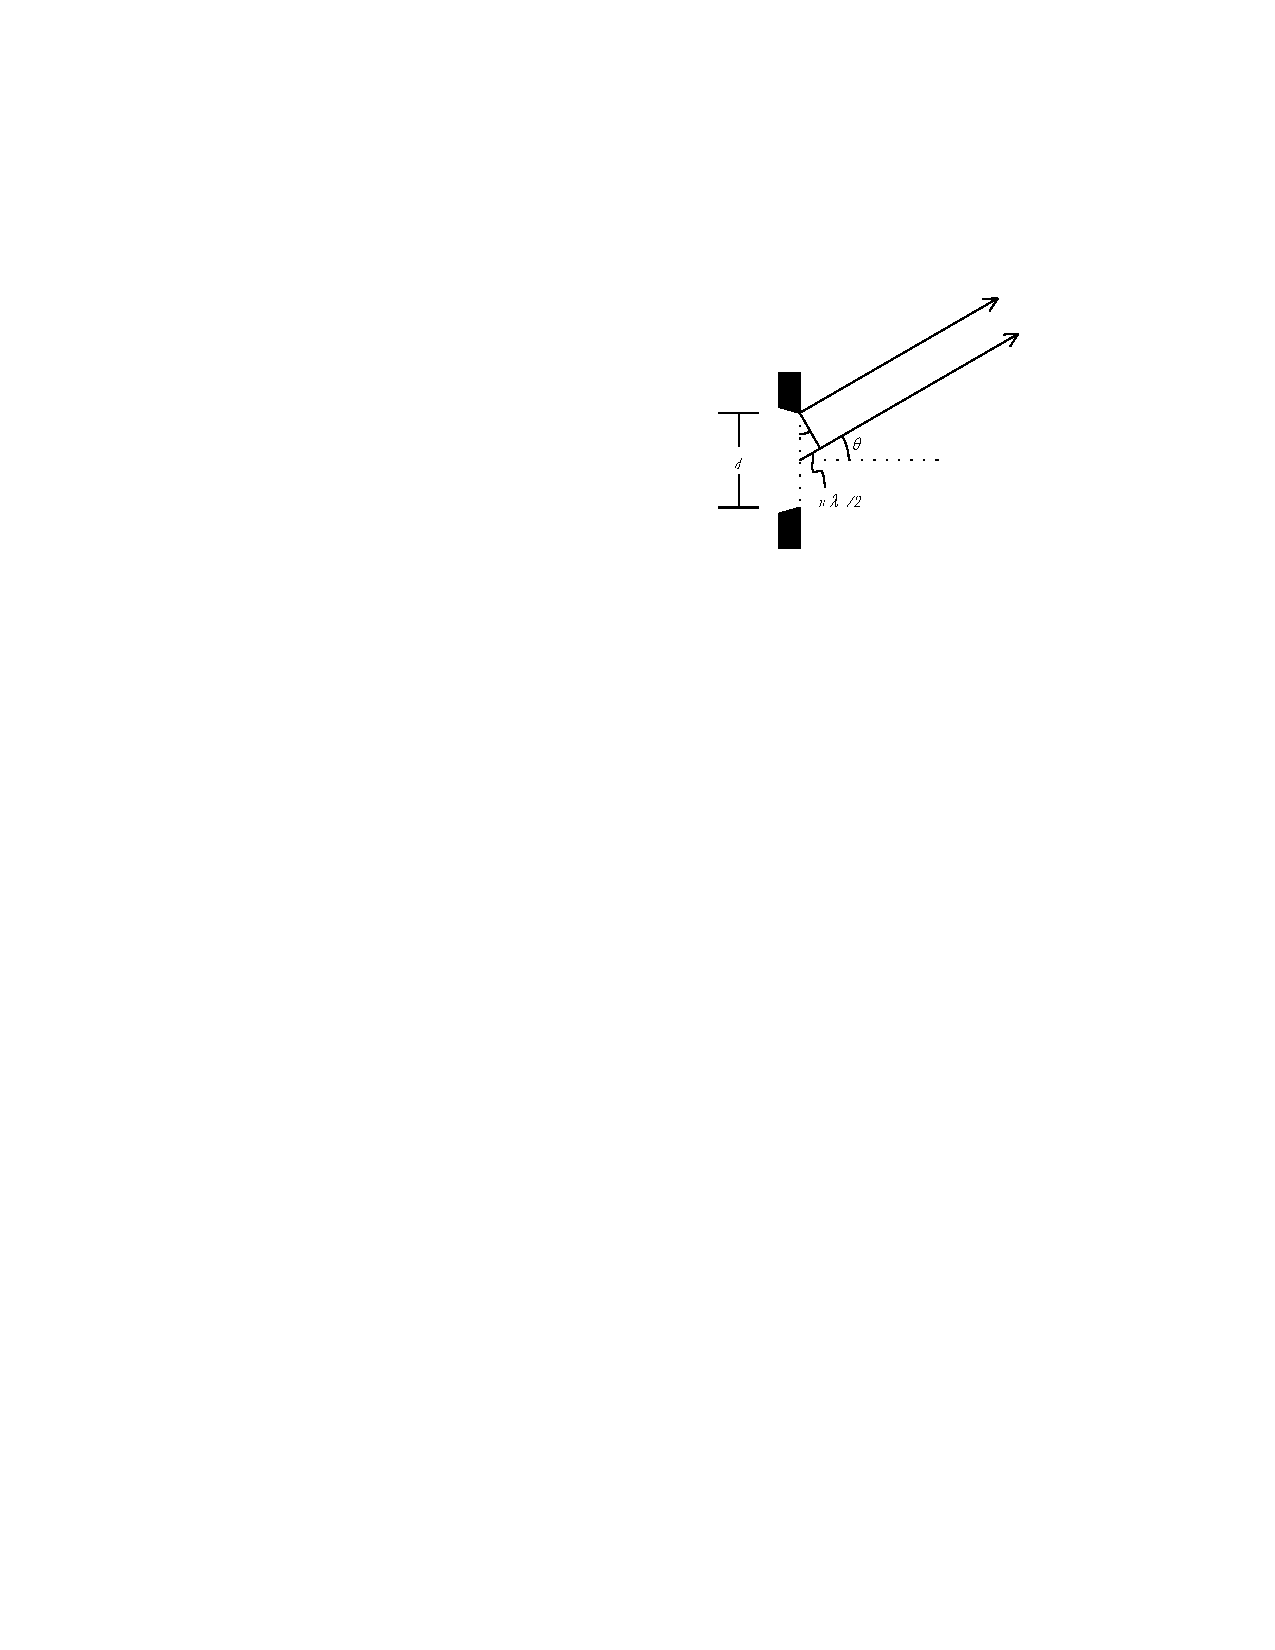
\includegraphics{Figure1SSD.pdf}
\end{wrapfigure}

1. \emph{Single-slit diffraction}. Let there be a narrow slit of width
$d$, illuminated uniformly along the axis perpendicular to the
plane of the slit. As in Huygens' treatment, consider the plane of the
slit to be populated by infinitely many centers of wavelets, expanding
in all forward directions. Thus the light beam will spread out as it
leaves the slit.


There will be some angle, say $\theta$, at which the wavelets that were
emitted from \emph{one edge} of the slit and from the \emph{center} of
the slit, respectively, will cover distances that differ by an integral
number of half-wavelengths and arrive together at some distant
point---where they will mutually cancel, being exactly out of phase with
one another. The innumerable remaining wavelets may be similarly paired
for mutual cancellation; so that the overall result will be a dark spot
at angle $\theta$ from the perpendicular axis.

In the right triangle thus formed with hypotenuse $d/2$ and one leg
an integral multiple of $\lambda/2$, the marked angle will be equal to
$\theta$ and will have sine given by

\begin{equation*}
\sin \theta = \frac{n\lambda/2}{d/2} = \frac{n\lambda}{d}.
\end{equation*}

Since $n$ is any integer, there will be alternating bands of
illumination and darkness for all angles up to 90$^\circ$ on either side of the
perpendicular axis. But in practice the greatest illumination is found
within the ``central maximum,'' that region bounded by the two minima
for which $n = 1$ (called ``first-order'' minima). Suppose these
minima appear at angles $\theta_1$ on either side of the axis. Then
$\theta_1$ will be the \emph{angular half-width} of the central maximum,
and will be given by

\begin{equation*}
\sin \theta_1 = \frac{\lambda}{d}.
\end{equation*}

2. \emph{Optical resolution}.\footnote{After Curtis Wilson, c. 1980.}
Consider points P$_1$ and P$_2$ on the surface of some object. Let their
angular separation be $\beta$, and let it be supposed that both points
emit or reflect light of wavelength $\lambda$. For the sake of
simplicity, we will let the aperture through which light is admitted to
the instrument be a slit of width $a$ (a circular aperture can be
analogously treated, but numerous complications arise for that case).
Light from each point forms its own independent diffraction pattern with
a central maximum flanked by pairs of minima. As shown in the previous
section 1, each central maximum will have an angular half-width equal to
$\theta_1$ such that

\begin{equation*}
\sin \theta_1 = \lambda/a.
\end{equation*}

Now the central maxima of the two patterns lie in the focal plane of the
instrument lens and (since rays passing through the center of a lens are
not bent) must be separated from one another by the angle $\beta$. But
as aperture \emph{a} is made smaller, the angular half-width of each
central maximum increases, until eventually $\theta_1 = \beta$---that
is, the central maximum of each pattern coincides with a first-order
minimum of the other pattern. The central bright maxima will then be
immediately adjacent to one another. Inspection of the sum of the two
intensity graphs under these conditions shows that instead of forming
two distinct bands, the central maxima will merge into a \emph{single
band}.

Someone viewing such an image through the instrument would be quite
unable to distinguish either of these maxima from the other; and thus
the points P1 and P2 would become \emph{indistinguishable}. No increase
of magnifying power, so long as the same aperture width is retained, can
remedy this limitation. However, if the aperture width $a$ is
increased even the slightest amount, so that the separation between the
two patterns increases by any degree at all, there will be found a dip
between the two maxima when the sum of the intensity graphs is plotted
as before. Thus, that the central maximum of each pattern shall coincide
with the first-order minimum of the other is a \emph{limiting condition}
for the resolution of the images of two points; it is called
\emph{Rayleigh's criterion}.

Heisenberg's equation (16) derives directly from
Rayleigh's criterion. For suppose $\theta_1 = \beta$ as described
above; that is, let
%
\begin{equation}
\sin \beta = \lambda/a. % eqn (1)
\end{equation}
%
Let the object distance be $R$, and suppose also that angle
$\beta$ is very small. Then $\Delta x$ is the chord of a circle with
center at the vertex of $\beta$, and so it very nearly equals the arc
which it subtends. This small arc equals $R\beta$ \ (radians);
while in its turn a very small angle $\beta$ (in radians) nearly equals
$\sin \beta$. This gives $\Delta x \approx R \times \sin\beta$, so that
%
\begin{equation}
\sin \beta \approx \Delta x/R . % eqn (2)
\end{equation}
%
From equations (1) and (2) it follows that
%
\begin{equation}
\frac{\Delta x}{R} = \frac{\lambda}{a}. % eqn (3)
\end{equation}
%


Similarly, the aperture of width $a$ located at distance $R$
from a point will subtend an angle $\varepsilon$ such that, if $\varepsilon$ is
very small,
%
\begin{equation*}
\sin \varepsilon \approx a/R,
\end{equation*}
%
from which

\begin{equation}
a \approx R \sin \varepsilon. % eqn (4)
\end{equation}

Substitution of equation (4) into equation (3) above yields
%
\begin{equation*}
\frac{\Delta x}{R} \approx \frac{\lambda}{R \sin \varepsilon}
\end{equation*}
%
which becomes Heisenberg's equation (16), when $R$ is canceled from
both sides. Q.E.D.

\newpage
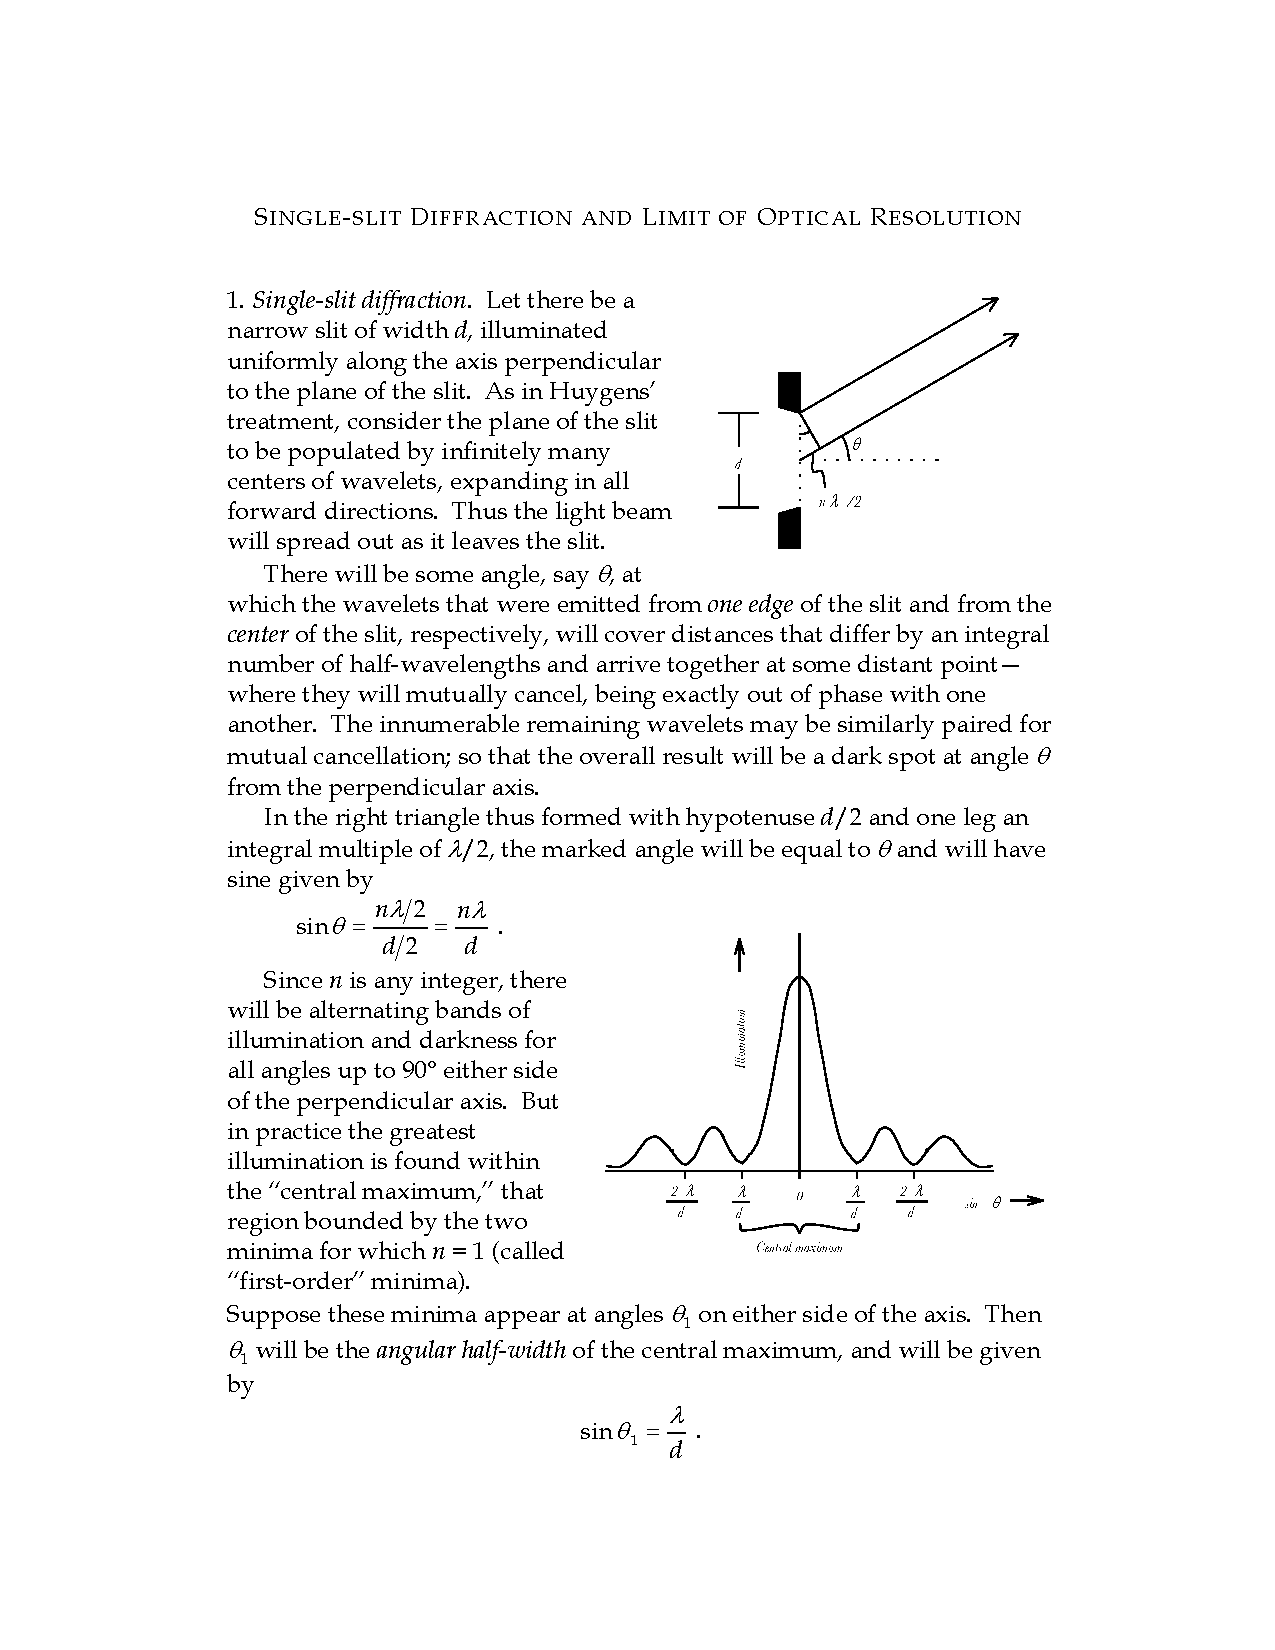
\includepdf[pages=-,pagecommand={},fitpaper=true]{Note_SSDiffraction}

\end{document}
